%\documentclass[9pt, twoside, openright, showtrims]{memoir}
\documentclass[10pt, a4paper, twoside, openright]{memoir}

\setstocksize{11in}{8in}
\settrimmedsize{9in}{7in}{*}
\settrims{0.7in}{.75in}
\settypeblocksize{7.5in}{6in}{*}
\setlrmargins{.85in}{*}{*}
\setulmargins{.5in}{*}{*}
\setheadfoot{\onelineskip}{2\onelineskip}
\setheaderspaces{*}{2\onelineskip}{*}

\checkandfixthelayout

\makeatletter
\DeclareOldFontCommand{\rm}{\normalfont\rmfamily}{\mathrm}
\DeclareOldFontCommand{\sf}{\normalfont\sffamily}{\mathsf}
\DeclareOldFontCommand{\tt}{\normalfont\ttfamily}{\mathtt}
\DeclareOldFontCommand{\bf}{\normalfont\bfseries}{\mathbf}
\DeclareOldFontCommand{\it}{\normalfont\itshape}{\mathit}
\DeclareOldFontCommand{\sl}{\normalfont\slshape}{\@nomath\sl}
\DeclareOldFontCommand{\sc}{\normalfont\scshape}{\@nomath\sc}
\makeatother

% \usepackage{xcolor, calc, graphicx, soul, fourier, verbments, makeidx, mflogo}
\usepackage{xcolor, calc, graphicx, soul, minted, makeidx, mflogo, 
  pstricks, minitoc, amsmath, amssymb, pst-poly, longtable, tikz}
\usetikzlibrary{shapes, arrows}
% Define block styles
\tikzstyle{decision} = [diamond, draw,
  text width=4.5em, text badly centered, node distance=3cm, inner sep=0pt]
\tikzstyle{startstop} = [rectangle, draw, 
  text width=5em, text centered, rounded corners, minimum height=2em]
\tikzstyle{line} = [draw, -latex']
\tikzstyle{cloud} = [draw, ellipse, node distance=3cm,
  minimum height=0.5cm]
\tikzstyle{io} = [trapezium, trapezium left angle=70, trapezium right
  angle=110, minimum width=0.5cm, minimum height=0.5cm, text centered, draw=black,
]
\tikzstyle{process} = [rectangle, minimum width=1cm, minimum height=0.5cm, text
  centered, draw=black]
\tikzstyle{arrow} = [->,>=stealth]

\let\footruleskip\undefined
\usepackage{fancyhdr}
\usepackage{fancyvrb}
\pagestyle{fancy}
%\usepackage[shellescape, latex]{gmp}
\showtrimson

\definecolor{niceblack}{rgb}{.1, .1, .1}
\definecolor{webred}{rgb}{.7,0,0}
\definecolor{webbg}{rgb}{1,.8,.2}
\definecolor{bootstrapurl}{rgb}{0,.5,.75}
%\definecolor{nicered}{rgb}{.347,.129,.149}
%\definecolor{nicegreen}{rgb}{.129,.447,.149}
%\definecolor{niceblue}{rgb}{0, 0, .6}
%\definecolor{niceyellow}{rgb}{1,1,.95}
%\color{niceblack}
\usepackage[colorlinks]{hyperref}
\hypersetup{%
  pdftitle={C Programming with C11},
  pdfauthor={Shiv S. Dayal},
  pdfkeywords={C, Programming},
  bookmarksnumbered,
  pdfstartview={FitH},
  urlcolor=niceblack,
  linkcolor=niceblack,
}%

\setlength{\tabcolsep}{10pt}
\renewcommand{\arraystretch}{1.5}

\renewcommand{\chaptermark}[1]{%
  \markboth{#1}{}}
\renewcommand{\sectionmark}[1]{%
  \markright{#1}{}}

\makeatletter
\newlength\dlf@normtxtw
\setlength\dlf@normtxtw{\textwidth}
\def\myhelvetfont{\def\sfdefault{mdput}}
\newsavebox{\feline@chapter}
\newcommand\feline@chapter@marker[1][4cm]{%
  \sbox\feline@chapter{%
    \resizebox{!}{#1}{\fboxsep=1pt%
      \colorbox{niceblack}{\color{white}\bfseries\sffamily\thechapter}%
  }}%
  \rotatebox{90}{%
    \resizebox{%
      \heightof{\usebox{\feline@chapter}}+\depthof{\usebox{\feline@chapter}}}%
              {!}{\scshape\so\@chapapp}}\quad%
  \raisebox{\depthof{\usebox{\feline@chapter}}}{\usebox{\feline@chapter}}%
}
\newcommand\feline@chm[1][4cm]{%
  \sbox\feline@chapter{\feline@chapter@marker[#1]}%
  \makebox[0pt][l]{% aka \rlap
    \makebox[1cm][r]{\usebox\feline@chapter}%
}}
\makechapterstyle{daleif1}{
  \renewcommand\chapnamefont{\normalfont\Large\scshape\raggedleft\so}
  \renewcommand\chaptitlefont{\normalfont\huge\bfseries\scshape\color{niceblack}}
  \renewcommand\chapternamenum{}
  \renewcommand\printchaptername{}
  \renewcommand\printchapternum{\null\hspace*{5.5in}\feline@chm[1cm]\par}
  \renewcommand\afterchapternum{\par\vskip\midchapskip}
  \renewcommand\printchaptertitle[1]{\chaptitlefont\raggedleft ##1\par}
}
\makeatother
\chapterstyle{daleif1}



\title{\HUGE{\textbf{Computer Programming with 
      GNU/Linux}}\\\vspace*{1cm}\Large{Vol. I}\\\vspace*{1cm}\HUGE{\textbf{C 
      Programming with C11}}\vspace*{2cm}}
\author{\vspace*{1cm}\LARGE{Shiv S. Dayal}}
\date{}

%\renewcommand{\ttdefault}{pcr}
%\renewcommand{\rmdefault}{ptm}
%\renewcommand{\rmdefault}{phv}
\renewcommand{\contentsname}{Table of Contents}
\makeindex
\begin{document}
\dominitoc
\dominilof
\dominilot
\maketitle
\thispagestyle{empty}
\pagestyle{empty}
\vfill
\newpage
\vspace*{7in}
Copyright, \copyright~ Shiv Shankar Dayal, 2011. All rights reserved.
\newpage
\vspace*{2in}
\begin{center}
  Dedicated to my family\\and Free Software Community
\end{center}
\newpage
\setcounter{page}{1}
\pagenumbering{roman}
\tableofcontents
\newpage
\listoffigures
\newpage
\listoftables
% \newpage
% \listofpyglistings
\newpage
\pagestyle{fancy}
\frontmatter
\setcounter{page}{1} 
\pagenumbering{roman}
\chapter{Preface}
I welcome you to this pdf version of 
\url{https://10hash.com/books/c/} which is a complete rewrite. That 
was my first attempt to write at such a large scale and therefore there were 
many deficiencies in that version which I hope have been countered and
corrected in this version. In the HTML version I had put a lot of emphasis on 
specification. However, the feedback which I got from some of my readers is 
that it has become complicated and is not suitable for beginners. After 
thinking over it I found that it is the order of chpaters which needs to be 
corrected and a lot more examples and exercises need to be there.

In this rewrite I will arrange the chapters in a different way. The empahsis on 
specification will be treated in the last part of book.

\section*{What this book contains?}
This book is about C programming language. In this book I have explained the
syntax of C programming language. But it is not only for learning about
language but how to learn to program using C programming language is also
there. In this book we will follow latest ISO specification of C which is
popularly known as C11.

\section*{Who should read this book?}
People interested in learning C should read this. Anybody can read this book
who has little background on Mathematics. I would say high school education is
sufficient for reading it. So this book is for both beginners and experts
alike. For experts advanced concepts have been presented and also a reference
to standard library has been given along with its usage.

\section*{How to read this book?}
Well, learning programming is like learning a new language and then solving
problems is like Mathematics. So the latter is more important as unless you can
solve the problem on pen and paper, you cannot solve the problems using
C. However, the focus of this book is to explain the features and syntax of C
programming language not on how to solve the problem. To get a good grasp
on the contents of the book one should read the theory first then look at the
examples given and try to understand and run them and in the end attempt
the problems. If you cannot solve the problems then lookup the solution and
try to understand. In case of any problem please log on to my personal
question/answer website \url{http://kunjika.libreprogramming.org/} to get
more help.

\section*{Acknowledgements}
I am in great debt of my family and free software community because both of
these groups have been integral part of my life. Family has prvided direct
support while free software community has provided the freedom and freed me
from the slavery which comes as a package with commercial software. I am
especially grateful to my wife, son and parents because it is their time which
I have borrowed to put in the book. To pay my thanks from free software
community  I will take one name and that is Richard Stallman who started all
this  and is still fighting this never-ending war. When I was doing the Algebra
book then I realized how difficult it is to put Math on web in HTML format and
why Donald Knuth wrote \TeX{}. Also, \TeX{} was one of the first softwares to
be released as a free software. HTML has not yet matured to represent
mathematical content. MathML is supported by Mozilla. Webskit browsers started
supporting  then dropped and I would refrain to comment on commercial browser's support which do not even comply to starndard because they think they are the standards tehmselves and others will bend to their will.

Now as this book is being written using \LaTeX{}~ so obviously Leslie Lamport
and all the people involved with it have my thanks along with Donald Knuth. I
use Emacs with Auctex and hope that someday I will use it in a much more
productive way someday.

I have used TikZ as a tool for drawing all the diagrams. It is a wonderful
package and works very nicely. I have great appreciation for its author Till
Tantau.

%For syntax highlighting I have used \texttt{Verbatim} \LaTeX{} package which
%uses \texttt{pygments} as its backend. You can modify it and make it look
%different both at \LaTeX{} and \texttt{pygments} level. Thanks to the
%respective package authors.

For errors and suggestion please email me at
\href{mailto:shivshankar.dayal@gmail.com}{shivshankar.dayal@gmail.com} where I
will try to respond to each mail as
much as possible. Please use your real names in email not something like
coolguy. As an alternative you can report it at
\url{https://10hash.com} where a question/answer website is maintained.
\begin{flushright}
Shiv Shankar Dayal\\
Nalanda,\\
India, 2015
\end{flushright}

\newpage
\mainmatter
\pagenumbering{arabic}
\chapter{Basics of C}
There are certain rules in every language, certain grammar which dictates the
way language will be spoken and written. It has a script to write
using. Similarly, programming languages have BNF (Backus-Naur Form)
context-free grammar. There are valid characters in a programming language and
a set of keywords. There are constructs to handle control flow, loops
etc. There are facilities provided by language to deal with numbers and strings
separately, to reuse the code and some basic data structures to facilitate
programming. However, programming language ruleset is very small compared
to a natural programming language. Also, when using natural programming
language like talking to someone or writing something the other person can
understand your intent but in programming you cannot violate rules. The grammar
is context-free. Compilers or interpreters cannot deduce your intent by reading
code. They are not intelligent. You make a mistake and it will refuse to listen
to you no matter what you do. Therefore, it is very essential to understand
these rules very clearly and correctly.

\section{The C Character Set}
The following form the C character set you are allowed to use in it:

\begin{verbatim}
[a-z] [A-Z] [0-9] ~ ! # % ^ & * ( ) - = [ ] \ ; ' , . / _ + { } | : " < > ?
\end{verbatim}
\index{character set}

This means along with other symbols you can use all English alphabets (both
uppercase and lowercase) and Arabic numerals. Symbols like \texttt{\$} and
\texttt{@} are not part of C's character set. But strings can contain any
these characters also. Strings are sequence of characters with double quotes
and double quotes iteself are escaped with \texttt{$\backslash$}. Also,
\texttt{\$} and \texttt{@} can also be value of characters. Characters are
values containing single characters withing single quotes. We will see more of
these in their individual sections. However, English is not the only
spoken language in the world. Therefore in other non-English speaking counties
there are keyboard where certain characters present in above set are not
present. The inventors of C were wise enough to envision this and provide the
facility in form of trigraph sequences. Given below is the trigraph sequence
table:

\begin{table}
 \begin{center}
 \caption{Trigraph Sequences}
\begin{tabular}{|c|c|c|c|c|c|}
\hline
\textbf{Trigraph}&\textbf{Equivalent}&\textbf{Trigraph}&\textbf{Equivalent}&\textbf{Trigraph}&\textbf{Equivalent}\\
\hline
??=&\#&??'&\textasciicircum&??!&|\\
\hline
??(&[&??)&]&??$<$&\{\\
\hline
??$>$&\}&??/&\textbackslash&??-&\textasciitilde\\
\hline
\end{tabular}
\end{center}
\end{table}
\index{trigraph sequences}

However, you should refrain from using trigraph sequences for portability 
reasons as suggested by GNU coding standards.

\section{Keywords}
The following are reserved keywords for C programming language which you are not 
allows to use other than what they are meant for:
\index{keywords}
\begin{table}[H]
 \begin{center}
  \caption{Keywords of C}
  \begin{tabular}{l l l l l}
    auto & break & case & char & const\\
    continue & default & do & double & else\\
    enum & extern & float & for & goto\\
    if & inline & int & long & register\\
    restricted & return & short & signed & sizeof\\
    static & struct & switch & typedef  & union\\
    unsigned & void & volatile & while & \_Bool\\
    \_Complex & \_Imaginary & &\\
  \end{tabular}
 \end{center}
\end{table}

These keywords are special in C as said and cannot be used for variable names 
or funciton names or otherwise other than in strings and comments.

\section{Identifiers}
The names which we give to our variables are known as identifiers. Something 
with which we identify the variables. As you have already seen what is allowed 
in C's character set but not all are allowed in an identifiers name. Only 
alphabets from English language both lowercase and uppercase, Arabic digits from 
zero to nine and underscore (\_) are allowed in an identifiers name. The rule 
for constructing names is that among the allowed characters it can only begin 
with only English alphabets and underscore. Numbers must not be first character. 
For example, \texttt{x, \_myVar, varX} and \texttt{yourId78} are all valid 
names. However, take care with names starting from underscore as they are mostly 
used by different library authors. Invalid identifier examples are \texttt{9x, 
my\$} and \texttt{your age}. Please read this section carefully and make sure 
understand the rules for naming identifiers. Later at the end of chapter there 
are some simple problems to practice with.

\section{Programming}
Let us revisit our first program and try to understand what it does. Here I am 
giving code once again for quick reference:

\begin{minted}{c}
// My first program
/* Description: This program does nothing.*/

#include <stdio.h>

int main(int argc, char* argv[])
{
  return 0;
}
\end{minted}

You can now issue a command as \texttt{\$gcc nothing.c} where 
\texttt{nothing.c} is the filename by which you saved the source code. Note 
that \texttt{\$} is the prompt not part of command itself. Then you can do an 
ls and you will find that \texttt{a.out} is a file which has been produced by 
clang. Now you can run this program by saying \texttt{\$./a.out} and nothing 
will happen. But if you type \texttt{\$echo \$?} then you will find that 0 is 
printed on screen which is nothing but 0 after \texttt{return} of our program.

As you can see this program does almost nothing but it is fairly complete 
program and we can learn a lot from it about C. Let us try to dissect it line
by line. The first line is a comment. 
Whenever C compiler parses C programs and it encounters \texttt{//} it ignores 
rest of line as code i.e. it does not compile them. This type of single line 
comment were introduced in C99 standard and if your compiler is really old the 
compiler may give you error message about it. The second line is
also comments. Anything between \texttt{/*} and \texttt{*/} is ignored like 
\texttt{//}. However, be careful of something like \texttt{/* some comment */
  more comment */}. Such comments will produce error messages and your program
will fail to compile. The reason for this is when first \texttt{*/} is
encountered by parser or compiler it will complete its token for the comment
and then further portion which we intented to be part of comment will cause
syntax error. 

Comments are very integral part of programming. They are used to describe 
various things. You can write whatever you want. They may also be used to 
generate documentation with tools like doxygen. Typically comments should tell
what the program is doing not how. Sometimes how can be covered, when the logic
is really complex. One should be generous while commenting the code.

The next line is \texttt{\#include <stdio.h>}. \texttt{\#include} is a
preprocessor directive. The preprocessor directive is handled by the C
preprocesor which is handled by C preprocessor which looks in four directories
for include files. The include filename comes after \texttt{\#include} either in
angular brackets or double quotes. The C preprocessor looks for these at four
different places at least out of which one or posiibly two is of interest for
now as we are dealing with angular brackets. Depending on the way your compiler
is installed the file \texttt{stdio.h} may be in \texttt{/usr/include} or
\texttt{/usr/local/include} but then again it may be in a non-standard path
also although possibility of that is very less and then it is controlled by
parameters whose discussion is beyond the scope of book. Let us say
\texttt{stdio.h} is present in either of aforementioned directories then the C
preprocessor will copies the contents and pastes them in source file along the
way putting \texttt{\#line} macros which are used for debugging
purposes. \texttt{\#line} macro is discussed later in the chapter which deals
with macros. You can see the output of C preprocessor by typing \texttt{\$gcc
  -E nothing.c} since it will scroll a lot on you terminal you can use a pager
like \texttt{less} to read it. The \texttt{-E} tells \texttt{gcc} to just allow
preprocessoing and not compile and link the file.

I have recorded a video on basics of compilation which you can see at
\url{http://www.youtube.com/watch?v=ARsoVgknRU0}.

Next line is \texttt{int main(int argc, char* argv[])}. Now this is very special
function. Every complete executable(shared objects or dlls or archive
libraririe do not have main even though they are C programs) C program will
have one main function unless you do assembly hacking. This function is where
the programs start. The first word \texttt{int} is a keyword which shirthand
for integer. This signifies the return type of function. \texttt{main} is the
name of the function. Inside parenthesis you see \texttt{int argc} which tells
how many arguments were passed to program and is short form of argument
count. While \texttt{char* argv[]} is a pointer to array which we will see
later. For now let us just remember that it holds all the arguments to the
program including the program name.

Next is a brace. The scope in C is determined by braces. Something outside any
brace has global scope (we will see these later), something inside first level
of brace has function or local scope. Something inside second or more level of
braces have got that particular block scope. Scope here means that when there
will be a closing brace that particular variable which is valid in that scope
will cease to exist. However, we do not have to worry about that yet as we do
not have any variable. Just note that a corresponding closing brace will be the
end of main function. For every opening brace which starts a scope a closing
brace is mandatory.

Next line is \texttt{return 0;} This means whoever has called \texttt{main()}
will get a 0 as \texttt{return} is returning 0. In this case, receiver is the
shell or operating system 
which has invoked the very program. The semicolon is called the terminator and
used also on Java or C++ for example. The very requirement of semicolon is to
terminate the statement and move on to next statement.

However, the program shown does not do much. Let us write a program which has
some more functionality and we can explore more of C. So here is a program
which takes two integers as input from users and presents their sum as
output. Here is the program:

\begin{minted}{c}
// My second program
// Author: Shiv S. Dayal
// Description: It adds two numbers

#include <stdio.h>

int main()
{
  int x=0, y=0, sum=0;

  printf("Please enter an integer:\n");
  scanf("%d", &x);

  printf("Please enter another integer:\n");
  scanf("%d", &y);

  sum = x + y;

  printf("%d + %d = %d\n", x, y, sum);

  return 0;
}
\end{minted}
and the output is:
\begin{verbatim}
shiv@shiv:~/book/code$ ./addition
Please enter an integer:
7
Please enter another integer:
8
7 + 8 = 15
shiv@shiv:~/book/code$
\end{verbatim}

Note that \texttt{shiv@shiv:~/book/code\$} is the prompt.

Let us discuss new lines one by one. The line \texttt{int x=0, y=0, z=0;} is
declaration and definition or initialization of three ints. \texttt{int}
keyword in C is used to represent integers. Now we have three integers with
there values set to 0. Note that how the variables are separated by commas and
terminated by semicolon(as we saw in last program also). We could have also
written it like this:

\begin{minted}{c}
int x;
int y;
int z;

x = 0;
y = 0;
z = 0;
\end{minted}

or

\begin{minted}{c}
int x, y, z;

x = y = z = 0;
\end{minted}

However, the first method is best and most preferred as it prevents use before
definition. \texttt{int} is a data-type in C. \texttt{x, y,} and \texttt{z} are
called variables of type \texttt{int}. This means that the size of these
variables will be same as \texttt{int}. Note that 
C is a statically typed language and all types have predefined memory
requirements. In cour case, \texttt{int} requires 4 bytes on 32-bit and 64-bit
systems but 2 bytes on 16-bit systems.

Here I have created a video about variables of C which you can see at
\url{http://www.youtube.com/watch?feature=player\_embedded\&v=6whuGZwv2-k} and
you can watch another about \texttt{printf} and \texttt{scanf} at
\url{http://www.youtube.com/watch?feature=player\_embedded\&v=U3jCSTR7Ulo}.

Let us learn a bit about \texttt{printf}. This function is declared in
stdio.h. The prototype of \texttt{printf()} is

\begin{minted}{c}
int printf(const char *restrict format, ...);
\end{minted}

The first argument format is what we have in first two function calls. The
second is a \texttt{...} which means it can take variable number of arguments
known as variable-list. We have seen this in the third call.This means it will
take a string with optional variable no. of arguments. The string is called the
format-string and determines what can be printed with supplied arguments. These
\texttt{...} are used to supply variable no. of arguments. In the first two
\texttt{printf()} statements we just print the format-string so that is
simple. However, in the last one, we have format as \texttt{\%d} which
signifies a decimal integer. The integers printed are in the same order in
which they were supplied.

\texttt{scanf()} is scan function which scans for keyboard input. As by now you
know that \texttt{\%d} is for decimal integer but we have not said \texttt{x}
or \texttt{y}. The reason is \texttt{x} and \texttt{y} are values while
\texttt{\&x} and \texttt{\&y} are the addresses of \texttt{x} and \texttt{y} in
memory. \texttt{scanf()} needs the memory address to which it can write the
contents to. You will see \texttt{\&} operator in action later when we deal
with pointers. Just remember for now that to use a simple variable with
\texttt{scanf()} requires \texttt{\&} before its name.

Till now we have just seen only \texttt{int} data-type but then there are more
data types for other types of numbers, characters and strings. Let us see them
one by one.

\section{Data Types}
What are data types? Why C needs data types? C is a statically typed language
that is every variable has a type associated with it. These types determine
what kind of values these variables can hold and how they will be interpreted.
When everything is a voltage level why not just deal with 0s and 1s? The answer
is simple. You need to abstract and segregate how much is required. For
example, say you are given a sequence of 0s and 1s how much can you work with
them. We as humans are not very versed with 0s and 1s. Also, say we encode
character `A' for 10101 will it be easy for you to see A or numbers. Also,
numbers range from $-\infty$ to $\infty$. Also, since C is statically typed the
sizes of data types have to be known at compile time. There are four types of
data types. Integral, floating-point, arrays and pointers. Here, I will deal
with the two former types and leave latter two for later. The integral types
are \texttt{char, short int, int, long} and \texttt{long long} and
floating-point types are \texttt{float, double} and \texttt{long
  double}. \texttt{signed} and \texttt{unsigned} are sign modifiers which also
modified the range of data types but do not affect their memory
requirements. By default all basic data types are \texttt{signed} in nature and
you must qualify you variables with \texttt{unsigned} if you want that
behavior. \texttt{short} and \texttt{long} are modifiers for size which the
data type occupies but I consider them as different types because memory
requirements are different. The ranges of integral data types directly reflect
their memory requirements and if you know how much memory they are going to
occupy you can easily compute their ranges. The range of floating-point comes
from IEEE specification. IEEE standard document 754 governs the binary
representation of floating point numbers which you can read at
\url{http://www.eecs.berkeley.edu/~wkahan/ieee754status/IEEE754.PDF}. This is
not available from IEEE website itself as they sell the specification's
electronic copies.

Let us write a program to find out ranges for integral data types:

\begin{minted}{c}
// Description: It gives ranges of integral data types

#include <stdio.h>
#include <limits.h>

int main()
{
  printf("Size of char is..........%d\n", sizeof(char));
  printf("Size of short int is.....%d\n", sizeof(short int));
  printf("Size of int is...........%d\n", sizeof(int));
  printf("Size of long is..........%d\n", sizeof(long));
  printf("Size of long long is.....%d\n", sizeof(long long));
  printf("Size of float is.........%d\n", sizeof(float));
  printf("Size of double is........%d\n", sizeof(double));
  printf("Size of long double is...%d\n", sizeof(long double));c

  return 0;
}
\end{minted}

Here \texttt{sizeof} is a compile time operator which computes size of any type
passed to it as an argument. So it is computing sizes of all the data types as
shown in the program. The output is given below:

\begin{verbatim}
Size of char is..........1
Size of short int is.....2
Size of int is...........4
Size of long is..........8
Size of long long is.....8
Size of float is.........4
Size of double is........8
Size of long double is...16
\end{verbatim}

Please note that the output shown is on 64-bit machine and it will be different
on 32-bit machines.
%\chapter{Console I/O}
IO stands for input/output. C provides only mechanism to interact through
console using its standard library. C does not provide ways to have GUI
although that is possible with various GUI libraries most notable being
GTK. However, discussing about GTK is out of scope of this book. In this
chapter we will focus on console output facilities of C because any program we
write at this stage will be meaningless if it has no input/output. Typically
when we interact with a C program we give input using keyboard which is also
referred as \texttt{stdin} stream. The output is monitor or \texttt{stdout}
stream. There is one more stream \texttt{stderr} which is generally redirected
to monitor or a log file. For historical reasons these are known as
\texttt{FILE} stream which represents the datatype of these
streams. \texttt{FILE} is capable of representing other streams which are disk
based for example a file on your hard drive. There are more type of input
devices on a modern computer. For example, network i/o is there. Whenever you
browse web or download a file through your intenet connection network i/o comes
into play. There is an opengroup
which specifies functions for network related functions. Operating systems
like GNU/Linux are POSIX compatible which defines how network i/o will be
used. Even a printer is a special output device, a camera input, speakers
output, microphone input and so on. In this books we are concerned with
keyboard input, output on monitor and i/o using files. Other types of i/os are
out of scope of this book.

However, before we go on with i/o I would
like to present C's memory model which will be needed by our discussion of i/o
related functions. However, if things do not make sense even then please go
through it and come later to understand more. 

\section{C's Memory Model}
As you may be knowing RAM(random acess memory) is the area which is used as
primary memory. Whenever we execute a program the first thing which happens is
that it gets loaded into memory. Now a binary program becomes a process when it
is running i.e. a running program is referred as process. All processes have
memory area divided into different portions. These portions are known as data
segment, stack and code or text segment. Dats segement is further split in
three parts; initialized data segment, uninitialized data segment or BSS which
is name after an ancient assembler Block Started by Symbol and
heap. Initialized data segment contains initialized global variables and static
variables. For uninitialized data segment it is same as above just that the
variables are not initialized explicitly but implicitly to zero.

Heap is the largest area of memory used for dynamic memory allocation. As
you will see later that you can manage heap using \texttt{malloc(), calloc(),
realloc(),} and \texttt{free()}. Note that operating system does not manage memory
allocated for you on heap. You, the programmer, are responsible for allocating and
freeing up memory in area. If heap gets full os will use virtual memory or swap
space on hard disk. Objects allocated on heap persist across function
calls. However, there are some very nasty problems, which, come in picture when
you use heap. There are several of them. You may forget to allocate memory and
may dereference unallocated pointer. You may have initialized it to
\texttt{NULL} and try to dereference that. You may allocate and free twice. You
forgot to set pointer to \texttt{NULL} after freeing it. And last but not the
least you loose all pointers to the memory area before you can free. The nature
with this particular problem is that if your program is going to run for long
time then it is going to consume more and more memory. Because of its nature it
is known as memory leak. It is very difficult to detect such problems in code
which does not run for long periods of time. Our friend valgrind will come to
help up with this problem. When a memory leak happens it eats up RAM slowly and
then operating system has to use virtual memory as explained above. In a
nutshell, I will say that heap means you have to manage it.

\begin{figure}[t!]
\begin{center}
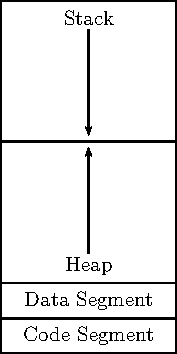
\includegraphics{figs/mem_model.pdf}
\end{center}
\caption{Memory model of a C program}
\end{figure}

Stack is relatively simple. All non-static and non-register variables go on
stack if not allocated dynamically. Stack variables do not retain there value
across function calls unless
they are passed as pointers. Also, when they go out of
scope, that is the scope in which they were declared ends, they will be kind of
lost. The way in which stack frame moves the same area will be used for new
variables. However, stack is very limited (compared to heap) and in deeply
nested function calls or recursion (you will see these in Functions chapter)
stack may get full and program may crash. The reason for crashing is that
operating system will not use virtual memory but will do a segmentation fault
in its place. GNU/Linux allow its users to modify the stack size by ulimit
command. Note that stack and heap are adjacent in memory and grow in opposite
direction.

Code segment or text segment is an area where the executable instructions of
program reside. It is typically constant and read-only area unless your system
allows self-modifying code. Following diagram shows the memory layout.

Note that this memory model not only applies to C but any process.

Now we will look at those functions, which, allow us to do console i/o. We will
begin with our familiar friends; printf and scanf.

\section{printf}
The prototype of \texttt{printf} is given by

\begin{Verbatim}[frame=single]
int printf(const char* fmt, ...);
\end{Verbatim}

Let us take a minute to understand this as we have not yet covered
functions. The first word is \texttt{int} which denotes the return type of the
\texttt{printf} function. This is no. of characters printed. Then we have name
of the function. \texttt{fmt} is the format string of type \texttt{const
 char}. In C, strings are either character arrays or character pointers. Here,
const means \texttt{printf} will not modify the format string. The ... means
variable no. of arguments, which, can be 0 also to be supplied to
\texttt{printf}.

\texttt{printf} is a string based output function that is It writes character
strings to \texttt{stdout}. The data which has to be written is formatted by
format string as shown previously. After the format specifier it expects as
many arguments as specified in format string. The characters which are not
like, say \texttt{\%d} for example, arecalled ordinary characters. These are
simply copied to output stream, which, is stdout for printf. The \texttt{\%d}
like conversion charcaters are known as conversion specification or format
specifiers. Each conversion specification should be augmented with one one
argument. The results are undefined if there are insufficient arguments for the
format. If extra arguments are given the excess arguments will be evaluated but
are otherwise ignored. However, there is a big problem here! There is no
type-safety. In general compiler will warn you about it and you, the
programmer, are responsible for giving correct format string, correct no. of
correct type of arguments. Consider the following program for example:

\begin{Verbatim}[frame=single]
#include <stdio.h>

int main()
{
  printf("%d %d\n", 3, 8);

  //do not mess it. undefined behavior
  printf("%d %d\n", 5);

  //extra arguments ignored
  printf("%d %d\n", 3, 5, "hello");

  //legal because char is integer type
  printf("%d\n", 's');

  //wrap around of integer as char
  printf("%c\n", 836);

  //do not mess with type-safety
  int i = printf("%d\n", "hello");
  prinf("%d\n", i);

  return 0;
}
\end{Verbatim}

now that if you give the command like \texttt{gcc -Wall printf.c} where
\texttt{printf.c} is the name of the ile then you will be shown following
warnings:

\begin{Verbatim}[frame=single]
printf.c: In function 'main':
printf.c:8:3: warning: format '%d' expects a matching 'int' argument [-Wformat=]
   printf("%d %d\n", 5);
   ^
printf.c:8:3: warning: format '%d' expects a matching 'int' argument [-Wformat=]
printf.c:11:3: warning: too many arguments for format [-Wformat-extra-args]
   printf("%d %d\n", 3, 5, "hello");
   ^
printf.c:11:3: warning: too many arguments for format [-Wformat-extra-args]
printf.c:20:3: warning: format '%d' expects argument of type 'int', but
argument 2 has type 'char *' [-Wformat=]
   int i = printf("%d\n", "hello");
   ^
printf.c:20:3: warning: format '%d' expects argument of type 'int', but
argument 2 has type 'char *' [-Wformat=]
\end{Verbatim}

Clearly this is not a good sign for any program. A program should compile
cleanly. In our case \texttt{gcc} is generating binary even though there are
warnings. You can make \texttt{gcc} generate more warnings by issuing a
\texttt{-Wall} flag. You can also treat all warnings as errors by passing
\texttt{-Werror} to \texttt{gcc}. These two options will ensure that your code
has no warnings. Now let us move to output and try to understand it. The output
on my system is as given below. It may differ on your system:
\\\\\texttt{3 8\\
5 8\\
3 5\\
115\\
D\\
134514119\\
10\\\\}
First \texttt{printf} is correct as expected. The second line causes undefined
behavior. You may think it is the previous 8 but believe me it is not
guaranteed that it will always the case. Ii is \textbf{UNDEFINED}. Third
\texttt{printf} is also fine in the sense that extra argument is
ignored. Fourth and fifth are normal. Sixth is again a big problem. You are
trying to print a decimal integer while argument is a character string. There
is no way for compiler to determine that what should be printed which will fit
on standards.

A full detail of all conversion specification is given in specification at \S(iso.7.21.6).

In real-world most of the time the conversion specifiers are kept simple. Given
below is a sample program showing some of the things given above:

\begin{Verbatim}[frame=single]
#include<stdio.h>

int main()
{
  int i   = 343456;
  float f = 123;
  long double ld = 78939.9347;

  printf("% d\n", i);
  printf("%+d\n", i);
  printf("%#o\n", i);
  printf("%#f\n", f);
  printf("%-08i\n", i);
  printf("%08i\n", i);
  printf("%8i\n", i);
  printf("%hhi\n", i);
  printf("%hi\n", i);
  printf("%li\n", i);
  printf("%lli\n", i);
  printf("%ji\n", i);
  printf("%zi\n", i);
  printf("%ti\n", i);
  printf("%8.8f\n", f);
  printf("%8.8Lf\n", ld);

  return 0;
}
\end{Verbatim}

The output of the above program is:
\\\\\texttt{ 343456\\
+343456\\
01236640\\
123.000000\\
343456\\
00343456\\
  343456\\
-96\\
15776\\
343456\\
4638355772471066016\\
4638355772471066016\\
343456\\
343456\\
123.00000000\\
78939.93470000\\\\}
We will keep seeing more conversion specifiers being used as we progress
through this book.

\section{scanf}
It scans \texttt{stdin} or keyboard for input. Its signature is same as that of
\texttt{printf()}. It reads bytes from keyboard input, interprets them
according to format string. It also expects a set of pointer arguments as
opposed to values for printf(). The pointers indicate where the interpreted
data from the input will be stored. The result is \texttt{UNDEFINED} if there
are less number of pointer arguments than the number of conversion specifers in
format string. Excess arguments will be evaluated but ignored. The format
string can have only white-space characters or an ordinary character (neither
`\%' nor a white-space character) or a conversion specification. Each
conversion specification is introduced by `\%', after which the following
appear in sequence.

For now if you do not understand what is a pointer then let us have a simple
definition for that. A pointer is a variable which stores a memory location
where the value will be stored.

Now that we have seen this description let us take a look at few examples.

\begin{Verbatim}[frame=single]
#include <stdio.h>

int main()
{
  char str[128] = {0};

  scanf("%s", str);
  printf("You entered:\n%s\n", str);

  return 0;
}
\end{Verbatim}

and the output is:
\\\\\texttt{\textbf{Hi! My name is Shiv.\\}
You entered:\\
Hi!\\\\}
It is certainly not the correct output. We had expected to see like: ``Hi! My
name is Shiv.''. What happend to input string after ``Hi!''. Well, in a form
given above for \texttt{scanf()} it will stop taking input after white-space
for character strings. For numerics it does not matter as it does not match the
format. For characters it is character-by-character so no confusion either. So
what if you want to have the entire string including white-spaces. Use
\texttt{[\^{}n]} as given below:

\begin{Verbatim}[frame=single]
#include <stdio.h>

int main()
{
  char str[128] = {0};

  scanf("%[^\n]s", str);
  printf("You entered:\n%s\n", str);

  return 0;
}
\end{Verbatim}

and the output is:
\\\\\texttt{\textbf{Hi! My name is Shiv.}\\
You entered:\\
Hi! My name is Shiv.\\\\}
What if you want to filter a string based on certain patterns. For example, a
charcater string does not contain more that a single space, English alphabets,
period and digits. To scan such a string you can define a pttern as program
given below shows:

\begin{Verbatim}[frame=single]
#include <stdio.h>

int main()
{
  char c[100]={0};

  scanf("%[ A-Za-z0-9!.]", c);
  printf("%s\n", c);

  return 0;
}
\end{Verbatim}

and the output is:
\\\\\texttt{\textbf{Hi! My name is Shiv! My phone no. is 1234. \%\^\$\&\*\\}
Hi! My name is Shiv! My phone no. is 1234.\\\\}
There is also a major problem associated with input and that comes when you
have characters involved. Consider the following program:

\begin{Verbatim}[frame=single]
#include <stdio.h>

int main()
{
  int   i = 0;
  float f = 0.0;
  char  c1 = '\0';
  char  c2 = '\0';
  char  c3 = '\0';

  printf("Enter an integer, a float and three character one by one:\n");

  scanf("%d", &i);
  scanf("%f", &f);
  scanf("%c", &c1);
  scanf("%c", &c2);
  scanf("%c", &c3);

  printf("You entered\n");
  printf("%d\n", i);
  printf("%f\n", f);
  printf("%c\n", c1);
  printf("%c\n", c2);
  printf("%c\n", c3);

  return 0;
}
\end{Verbatim}

and the output is:
\\\\\texttt{\textbf{2\\
3.4\\
s\\}
You entered\\
2\\
3.400000\\
\\
\\
s\\\\}
What is happening here is that newline entered by our RET key is getting
assigned to \texttt{c1} and \texttt{c3}. That is why the program accepted only
second character. The enter after \texttt{float f;} was assigned to \texttt{c1}
and the character entered to \texttt{c2} and then the RET newline to
\texttt{c3}. There is a very simple way to recover from this:

\begin{Verbatim}[frame=single]
#include <stdio.h>

int main()
{
  int   i = 0;
  float f = 0.0;
  char  c1 = '\0';
  char  c2 = '\0';
  char  c3 = '\0';

  printf("Enter an integer, a float and three character one by one:\n");
  scanf("%d", &i);
  scanf("%f", &f);
  scanf(" %c", &c1);
  scanf(" %c", &c2);
  scanf(" %c", &c3);

  printf("%d\n", i);
  printf("%f\n", f);
  printf("%c\n", c1);
  printf("%c\n", c2);
  printf("%c\n", c3);

  return 0;
}
\end{Verbatim}

The whitespace character shown will eat up all the white-space given after the
previous input. This concludes our discussion on \texttt{printf()} and
\texttt{scanf()}. Now we will move to another set of i/o functions which take
character string without filtering and print it to screen without
filtering. What I am going to discuss are \texttt{gets(), fgets(), puts()} and
\texttt{fputs()}.

All the following function's reference is present in \S(iso.7.21) which deals with
header `stdio.h`.

\section{Sting I/O Functions}
These functions are very simple compared to \texttt{printf(}) and
\texttt{scanf()}. They take a pointer to a character array or a character
pointer and fill it with input or print it to monitor. Note that
\texttt{gets()} and \texttt{puts()} work only with \texttt{stdin} and
\texttt{stdout} respectively while \texttt{fgets()} and \texttt{fputs()} work
with \texttt{FILE} streams i.e. other than \texttt{stdin} and \texttt{stdout}
they can also work with disk based files. Here is a sample program:

\begin{Verbatim}[frame=single]
#include <stdio.h>
#include <stdlib.h>

int main()
{
  char cStack[1024] = "";
  char *cHeap = (char*)malloc(sizeof(1024));

  gets(cStack);
  puts(cStack);

  cHeap = fgets(cHeap, 1024, stdin);
  fputs(cHeap, stdout);

  return 0;
}
\end{Verbatim}

and the output is:
\\\\\texttt{\textbf{Hi!\\}
Hi!\\
\textbf{Hello!\\}
Hello!\\\\}
First \texttt{``Hi!''} and \texttt{``Hello!''} are keyboard inputs. Do not
worry about array and pointer syntax at the moment. Just see the difference
between function calls. Their is a problem with \texttt{gets()} that it can
cause buffer overflow. If input is bigger than 1024 bytes including the null
terminator then buffer overflow will happen. Note how you can prevent it with
\texttt{fgets()} by specifying the number of characters you want to read. Rest
of input will be ignored by \texttt{fgets()}. This is a security hole and
therefore you should never ever use \texttt{gets()}.

\section{Character I/O Functions}
There are several functions for single character i/o. They are \texttt{getc(),
  putc(), getchar(), putchar(), fgetc()} and \texttt{fputc()}. Apart from
\texttt{getchar()} and \texttt{putchar()} rest can do any FILE stream-based
i/o. Let us have a simple program as they are mostly trivial.

\begin{Verbatim}[frame=single]
#include<stdio.h>

int main()
{
  char c ='';

  c = getchar();
  putchar(c);

  c = getchar();
  putchar(c);

  c = fgetc(stdin);
  fputc(c, stdout);

  c = getchar();
  putchar(c);

  c = getc(stdin);
  putc(c, stdout);

  return 0;
}
\end{Verbatim}

and the output is:
\\\\\texttt{\textbf{4\\}
4\\
\textbf{5\\}
5\\
\textbf{6\\}
6\\\\}
The first 4, 5 and 6 were keyboard inputs. Note the use of extra
\texttt{getchar()} and \texttt{putchar()} to handle the situation we faced
during \texttt{scanf()}.



\printindex
\backmatter
\end{document}
